\section{Fundamentals}
\label{gw_fundamentals}
GW are oscillations in spacetime, similar to electromagnetic
waves. We can start with the Einstein equation:

\begin{equation}
    G_{\mu\nu}= \frac{8\pi G}{c^4} T_{\mu\nu}.
\end{equation}

Since GW (mostly) propagate in the vacuum and we assume a small amplitude $|\delta g_{\mu\nu}| \ll 1$, we arrive at the following differential equation.

\begin{equation}
    T_{\mu\nu} = 0
\end{equation}
\begin{equation}
    \Rightarrow G_{\mu\nu} = 0
\end{equation}


We assume that the metric only has small linear perturbations. 
\begin{equation}
    g_{\mu \nu}(t, \vec{x}) = \bar{g}_{\mu \nu}(t) + \delta g_{\mu \nu}(t, \bar{x})
\end{equation}
\begin{equation}
   = \eta_{\mu \nu} + 2\kappa h_{\mu \nu}
\end{equation}
\begin{equation}
    \kappa = \frac{\sqrt{8\pi G}}{c^2} \approx 2.1 \cdot 10^{-41}\frac{\rm{s}^2}{\rm{kg}\,\rm{ m}}
\end{equation}
\begin{equation}
    |h_{\mu \nu}| << 1
\end{equation}
Here $\eta_{ \mu \nu}$ the Minkowski metric for flat spacetime.

We can solve the differential equation with the trace reverse tensor.

\begin{equation}
    \bar{h}_{\mu\nu} = h_{\mu\nu}-\frac{1}{2} \eta_{\mu\nu}h
    \label{trace_reverse}
\end{equation}

Here, $h$ is the trace of $h_{\mu\nu}$.

\subsection{Wave Equation}

If we want to describe the transport of energy and momentum by GW analytically, we can assume an asymptotically flat environment since the detector is at a far distance from the source. Then, we will consider Newtonian binaries in a circular orbit and only look at the non-relativistic regime. This will limit us to the inspiral phase, see Fig. \ref{GW_waveform} since the non-relativistic approximation only applies in that phase. Later though, we will see that for the implementation in the {\tt CLASS} code all the phases need to be modelled.

The linear perturbation $h_{\mu\nu}$ is a dimensionless bosonic tensor field and thus follows the massless field equation (\cite{van_holten_gravitational_2019}):

\begin{equation}
    \square h_{\mu\nu} -\partial_mu \partial^\lambda h_{\lambda\nu}-\partial_\nu\partial^\lambda h_{\lambda\mu}+\partial_\mu \partial_\nu h - \eta_{\mu\nu}(\square h-\partial^\kappa \partial^\lambda h_{\kappa\lambda})=-\kappa T_{\mu\nu}
\end{equation}

For the gauge transformation, we can impose the de Donder gauge condition:

\begin{equation}
    \partial^\mu h_{\mu\nu} = \frac{1}{2}\partial_\nu h_\mu^\mu .
    \label{de_donder}
\end{equation}

This simplifies the wave equation to the following form with the trace reverse tensor (\ref{trace_reverse}).

\begin{equation}
    \partial^\mu \underline{h}_{\mu\nu}=0
\end{equation}

\begin{equation}
    \Rightarrow \square \underline{h}_{\mu\nu}=-\kappa T_{\mu\nu}
\end{equation}

We can also choose $h$ to be traceless, which leads to $h$ and $\underline{h}$ coinciding.

\begin{equation}
    h = h_{\ \mu}^\mu := 0
\end{equation}
\begin{equation}
    \Rightarrow \underline{h}_{\mu\nu}=h_{\mu\nu}
\end{equation}
\begin{equation}
    \Rightarrow \underline{h} = \underline{h}_{\ \mu}^\mu =0
\end{equation}

\subsection{Free Field Modes}

Now, we can perform a Fourier decomposition of the linear perturbation.

\begin{equation}
    \underline{h}_{\mu\nu}(x) = \int \frac{d^4k}{(2\pi)^2} \epsilon_{\mu\nu}(k)e^{-ikx}
\end{equation}

\begin{equation}
    k=(\omega, \vec{k})
\end{equation}

The field equation is invariant under the following gauge transformation. 

\begin{equation}
    \epsilon '_{\mu\nu}=\epsilon_{\mu\nu}+k_\mu \alpha_\nu + k_\nu \alpha_\mu - \eta_{\mu\nu}k^\lambda \alpha_\lambda
    \label{epsilon_prime_gauge}
\end{equation}

Since $k$ is the wave vector and GW propagate with the speed of light, it has to be a light-like four-vector.

\begin{equation}
    k^2=0
\end{equation}

\begin{equation}
    \Rightarrow \epsilon_{\mu\nu}(k) = e_{\mu\nu} (k)\delta(k^2)
\end{equation}

To get a simplified amplitude form, we choose $\alpha$ from the gauge condition \ref{epsilon_prime_gauge} in such a way that we eliminate $e'_{00}, e'_{i0}$ and $e'_{ii}$. 

\begin{equation}
    \epsilon '_{\mu\nu}(k) = e'_{\mu\nu} (k)\delta(k^2) 
\end{equation}

For a wave propagating in z-direction, we will then get the following amplitude form.

\begin{equation}
    e'_{\mu\nu}(\omega, \vec{k})=
    \begin{pmatrix}
        0 & 0 & 0 & 0 \\
        0 & e_+(\omega) & e_\times(\omega) & 0 \\ 
        0 & e_\times(\omega) & -e_+(\omega) & 0 \\
        0 & 0 & 0 & 0
    \end{pmatrix}
\end{equation}

To illustrate plus and cross polarisations, Fig. \ref{polarisation} shows both over one period.

\begin{figure}[h]
    \centering
    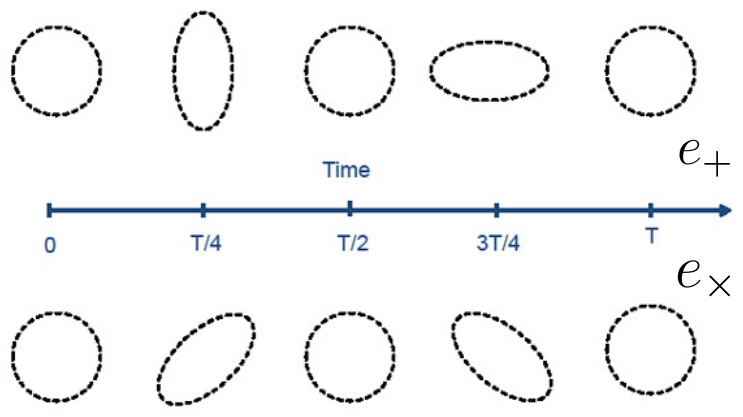
\includegraphics[width=0.4\linewidth]{Images/polarisations.png}
    \caption{Illustration of the plus and cross polarisations varying with time. The figure is taken from a lecture by Prof. Jan van Holten.}
    \label{polarisation}
\end{figure} 


Then, a plane wave in z-direction with plus polarisation would have the following expression, since the cross polarisation will be zero.
\begin{equation}
    h(z, t) = h_+ 
    \begin{pmatrix}
        0 & 0 & 0 & 0 \\
        0 &1 & 0 & 0 \\
        0 & 0 & -1 & 0 \\
        0 &  0 & 0 & 0
    \end{pmatrix}
    e^{i(k z-\omega t)}
\end{equation}

For a length of $L_0$ along the x-axis, it would oscillate in size in the
following way:
\begin{equation}
    L(t) = L_0 + \frac{h_+ L_0}{2} cos(\omega t).
\end{equation}

\subsection{Quadrupole Wave Emission}
If we have a source in a finite region of space, we can use the retardated Green's function to solve the wave equation. This is because the waves are causally related to the source $t> |\vec{x}'-\vec{x}|$.

\begin{equation}
    \square \underline{h}_{\mu\nu}=-\kappa T_{\mu\nu}
\end{equation}

\begin{equation}
    \Rightarrow \underline{h}_{\mu\nu}(\vec{x}, t) = \frac{\kappa}{4\pi} \int d^3 x' \frac{T_{\mu\nu}(\vec{x}', t-|\vec{x}'-\vec{x}|)}{|\vec{x}'-\vec{x}|}
\end{equation}

Then, we can assume that we are in the far field regime, such that $|\vec{x}| \gg |\vec{x}'|$.

\begin{equation}
    r:= |\vec{x}| \approx |\vec{x}'-\vec{x}|
\end{equation}

\begin{equation}
    \Rightarrow \underline{h}_{\mu\nu}(\vec{x}, t) = \frac{\kappa}{4\pi r} \int d^3 x' T_{\mu\nu}(\vec{x}', t-r)
\end{equation}

If we consider a localised source, the solution does not have a dynamical time component, i.e. $\partial_0 h_{0j} = 0$ (\cite{van_holten_gravitational_2019}).
Additionally to the de Donder gauge (\ref{de_donder}), we will now impose the traceless-transverse (TT) gauge, which implies transversality.

\begin{equation}
    r_i \underline{h}_{ij} = 0
\end{equation}

\begin{equation}
    h_{ii} = 0
\end{equation}

This gives us the following solution which is valid at a large distance in empty space.

\begin{equation}
    \underline{h}_{ij}(\vec{x}, t)=\frac{\kappa}{4\pi}(\delta_{ik}-\hat{r_i}\hat{r_k})(\delta_{jl}-\hat{r_j}\hat{r_l})\left(I_{kl}+\frac{1}{2}\delta_{kl}\vec{r}\; \underline{I} \; \vec{r}\right)
\end{equation}

$I_{ij}$ is the quadrupole moment of the total energy density:

\begin{equation}
    I_{ij}(t-r)= \int d^3x' \left(T_{ij} -\frac{1}{3}\delta_{ij}T_{kk} \right)T_{00}(\vec{x}', t-r) .
\end{equation}

\begin{equation}
    = \frac{1}{2} \partial_0^2 \int d^3x' \left(x_i' x_j' -\frac{1}{3}\delta_{ij}\vec{x}'^2 \right)T_{00}(\vec{x}', t-r) .
\end{equation}

The last equation follows since the time derivative is equal to the derivative with respect to the retardated time $u=t-r$.

\begin{equation}
    \partial_0 = \partial_u
\end{equation}
\begin{equation}
    \Rightarrow \partial_0^2T_{00}(\vec{x}', u) = \partial_0 \partial_i' T_{i0}(\vec{x}', u) = \partial_i'\partial_j' T_{ij}(\vec{x}', u)
\end{equation}
As mentioned earlier, we can perform a non-relativistic approximation for the inspiral phase. In this case, the energy density is dominated by the mass density. We can thus rewrite $\underline{h}_{ij}$ with the mass quadrupole moment. 


\begin{equation}
    I_{ij}=\frac{1}{2}\frac{\partial^2 Q_{ij}}{{\partial t^2}}
\end{equation}

\begin{equation}
    Q_{ij}(t-r)=\frac{1}{2} \int d^3x' \left(x_i' x_j' -\frac{1}{3}\delta_{ij}\vec{x}'^2 \right)\rho(\vec{x}', t-r)
\end{equation}

GW cannot form from a dipole mass distribution since that would require negative masses. However, if we have a quadrupole distribution with vacuum and masses (like a binary black hole for example), GW can be created.

The wave field for non-relativistic sources is thus:

\begin{equation}
    \underline{h}_{ij}(\vec{x}, t)=\frac{\kappa}{8\pi}(\delta_{ik}-\hat{r_i}\hat{r_k})(\delta_{jl}-\hat{r_j}\hat{r_l})\frac{\partial^2}{\partial t^2}\left(Q_{kl}+\frac{1}{2}\delta_{kl}\vec{r}\; \underline{Q} \; \vec{r}\right)
\end{equation}

\section{Stochastic Background}
The stochastic GW background consists of all sources that are too faint to be resolved individually, thus it is a superposition of many independent sources. The same source can contribute to multiple frequencies over time. 
The biggest background comes from astrophysical sources, like compact object mergers, but there is also a smaller cosmological background present. That one originates from early universe phenomena. 
To measure the background we need the correlation between two detector
outputs \cite{christensen_stochastic_2019}. If the noise between them is uncorrelated, it will average out over time and leave the background signal.
\begin{equation}
    \langle s_1 (t) s_2(t)\rangle \, = \, \langle(n_1(t) + h(t))(n_2(t) + h(t))\rangle
\end{equation}
\begin{equation}
    = \, \langle n_1(t) n_2(t)\rangle + \langle n_1(t)h(t)\rangle + \langle h(t)n_2(t)\rangle  + \langle h(t)h(t)\rangle  
\end{equation}
\begin{equation}
    \approx \, \langle h(t)h(t)\rangle 
\end{equation}
From there we can compute the root mean square of the strain.
\begin{equation}
    h_{rms}^2 = \langle \sum_{i,j} h_{ij} h_{ij}\rangle 
\end{equation}
\begin{equation}
    = \int_0^\infty df \, S_h (f)
\end{equation}
Here $S_h$ is the spectral density, from which we can derive the GW energy
density.
\begin{equation}
    \rho_{GW} = \int_0^\infty df \, S_h(f) \frac{\pi c^2 f^2}{8G}
\end{equation} 

The frequency-dependent monopole depends on this energy density. Here, we consider the observed frequency $f_o$.
\begin{equation}
    \bar{\Omega}_{AGWB}(f_o)=\frac{d\rho_{GW}}{df}
\end{equation}

The energy density parameter is the frequency-dependent monopole integrated over the logarithmic frequency.

\begin{equation}
    \Omega_{GW} = \int d\ln f \; \Omega_{GW}(f_o) 
\end{equation}
\begin{equation}
    \approx \int d\ln f \; \bar{\Omega}_{AGWB}(f_o)
\end{equation}

\subsection{Astrophysical}
GW can be created by different sources. Considering astrophysical sources, they can come from
merging binaries, bursts (e.g. from core-collapse supernovae) or continuous waves 
(e.g. from pulsars). 
The AGWB consists mostly of compact object mergers, which are mainly black holes and neutron stars. 

Anisotropy limits from LIGO:
(check for more current)
The LIGO anisotropy limit for the first observing run O1 published in 2017
was 
\begin{equation}
    \Omega_{2/3} = (4.4 \pm 6.4) \cdot 10^{-8} .
\end{equation}

This is compatible with zero, but an anisotropic background would indicate
a more interesting cosmology, which is why it would be important to disentangle
any anisotropic that could be observed.

The AGWB was detected for the first time this year (2023) using the pulsar time array NANOGrav \cite{agazie_nanograv_2023}. Pulsar time arrays use the fact that pulsars are very accurate clocks. They are rotating neutron stars that have a strong magnetic field and thus emit radio waves in very regular intervals. Since they are so stable, we can use these signals as accurate clocks. If there are any changes in the time of arrival of multiple pulsars, this could indicate a GW background. 
The NANOGrav experiment used a frequency range of $10^{-8.75} - 10^{-7.5}$ Hz. They assumed a GW energy density parameter proportional to $f^{-2/3}$, which is the case in the inspiral phase of binary black holes. \cite{phinney_practical_2001}
Using this, they find an integrated energy density $\Omega_{GW} = 9.3^{+5.8}_{-4.0}\cdot 10^{-9}$.


\subsubsection{Binary Black Hole Mergers}
\label{BBH_mergers}

A compact binary coalescence will produce a chirp-like GW signal, like in \ref{GW_waveform}. Both massive objects attract each other and decrease their orbit around each other in the inspiral phase. The potential energy is converted into a GW. After the inspiral phase, the merger and ringdown phases follow, where the new BH becomes axisymmetric and stops emitting GW. The frequency increases over time during all three phases.

The inspiral phase is the simplest to describe analytically, see \ref{gw_fundamentals}. However, in this work, we consider all three phases of the GW. We will see later that this is necessary to derive a frequency dependence.


In this work, we focus on binary black holes. Since most resolved events from LIGO/Virgo are binary black holes. In a recent analysis of the Gravitational Wave Transient Catalogue 3 (GWTC-3) by \cite{the_ligo_scientific_collaboration_population_2022}, they considered events with a false alarm rate of less than $\frac{1}{4}$ per year. Out of this sample of 67 events, 63 came from binary black holes, 2 from binary neutron stars and 2 from neutron star-black hole mergers.

If we consider the energy density parameter of the stochastic GW background, we see that binary black holes are present at frequencies up to around 1000 Hz, see Fig. \ref{BG_sources}. 

\begin{figure}[h]
    \centering
    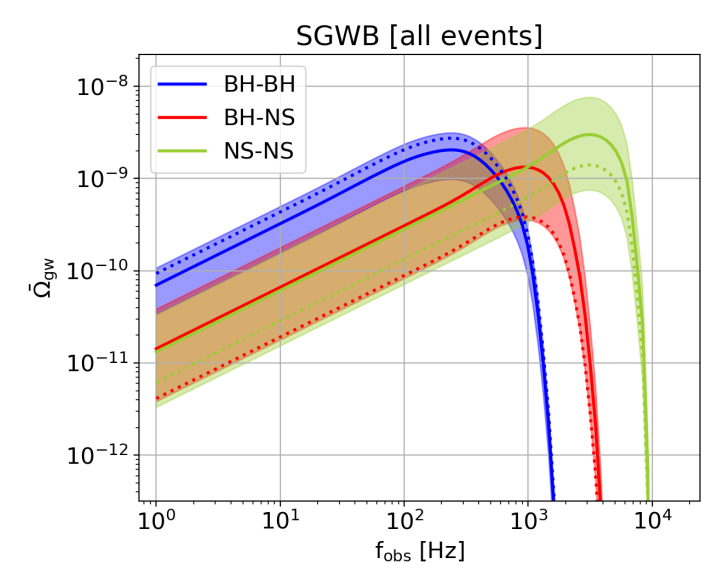
\includegraphics[width=0.7\linewidth]{Images/Capurri_GW_Background_monopole_sources.png}
    \caption{The GW energy density parameter as a function of frequency from 1 to 10,000 Hz. This shows the different contributions from BH-BH, NS-NS and BH-NS events. All curves are normalised to the local advanced LIGO/Virgo merger rate. The Figure is taken from Ref. \cite{capurri_intensity_2021}.} 
    \label{BG_sources}
\end{figure} 

In this figure, all three curves are normalised to the local merger rate from the advanced LIGO/Virgo detectors. Without this normalisation binary BH mergers dominate at most frequencies at which they are present. We can see that for the frequency range of $1-1000 Hz$, it is reasonable to only consider BBH in our analysis since they are the most present source. However, the applied formalism for the frequency dependence can be generalised to a system of a BH and a neutron star or a system of two neutron stars.

\begin{figure}[h]
    \centering
    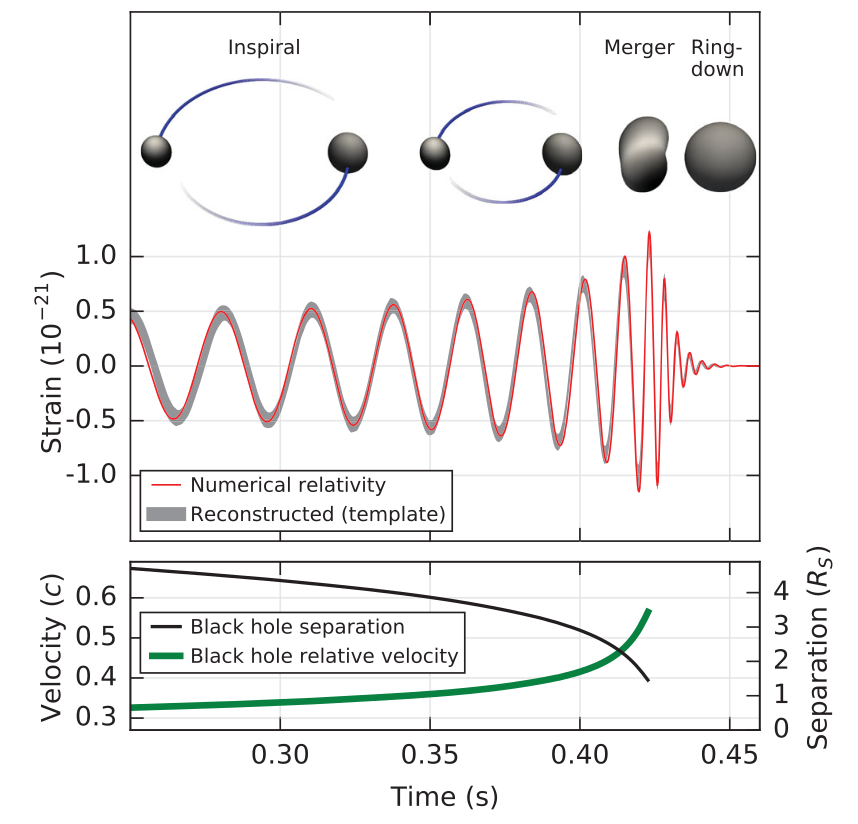
\includegraphics[width=0.7\linewidth]{Images/waveform_abbott_complete.png}
    \caption{The different stages of a BBH merger with the corresponding waveform, here an illustrative estimate of GW150914. The Figure is taken from Ref.\ \cite{abbott_observation_2016}.}
    \label{GW_waveform}
\end{figure} 

From the waveform, we can extrapolate black hole properties, like the chirp mass and the spin. 

\begin{equation}
    \mathcal{M}_c = \frac{(m_1m_2)^{3/5}}{(m_1+m_2)^{1/5}}
\end{equation}

The frequency is determined by the total mass. 
The waveform can be decomposed into harmonic, where the quadrupole ($(\ell, m)=(2,2)$) is naturally the dominant one. 
(insert from Bonn lectures?)


\subsubsection{Dipole}
The cosmological principle says, that the universe is isotropic and homogeneous on large scales. GW are one mode of testing this further. If we find anisotropies in the GW background, other than the kinematic dipole and shot noise, this would be evidence against the principle.
The kinematic dipole arises from the observer motion with respect to the large-scale structure rest frame. More GW events should be detected in the direction in which we move, and fewer in the opposite direction. Shot noise comes from stochastic fluctuations in the background, which follow a Poisson distribution.

The GW density contrast can be written with an integration over the window function, which weights the contributions in the redshift domain.

\begin{equation}
    \delta(f_0, \hat{n}) = \frac{\Omega(f_0, \hat{n})-\overline{\Omega}(f_0)}{\overline{\Omega}(f_0)}
\end{equation}
\begin{equation}
    = \int dz \; W(f_0, z) \; \Delta(f_0, \hat{n}, z)
\end{equation}

\subsection{Cosmological}
The major contributions to the cosmological GW background are primordial
black holes and GW from phase transitions and inflation.
Schulze et al. \cite{schulze_gw_class_2023} computed the angular power spectrum of this background using a modified version of CLASS \cite{blas_cosmic_2011} called {\tt GW\_CLASS}.
Bubbles of a phase can form in a universe which is in an older phase. In there, magnetohydrodynamic (MHD) turbulence can also produce GW.
TODO: PBH shortly
Using this code, one can choose a source of this background and compute the associated angular power spectrum. Here, we use the signal from the expected inflationary GW background with a blue tilt. So, we will have a stronger background at higher frequencies compared to lower frequencies. 

\subsubsection{Inflation}

A period of inflation in the early universe solves two important cosmological problems, namely the flatness and the horizon problem. The flatness problem arises when we assume radiation domination followed by matter domination which is followed by $\Lambda$ (the cosmological constant) domination. The spatial curvature density parameter is measured to be very low. 
\begin{equation}
    |\Omega_k| = \frac{\rho_k^{\rm{eff}}}{\rho_{crit}} < 10^{-2}
\end{equation} 
On the other hand, the radiation energy density parameter is of an even lower order.
\begin{equation}
    |\Omega_r| = \frac{\rho_r}{\rho_{crit}} \in \mathcal{O}(10^{-4}) 
\end{equation}

Now the effective curvature energy density $\rho_{k}^{\rm{eff}}$ scales like $a^{-2}$, while the radiation energy density $\rho_{r}$ scales like $a^{-4}$, with the scale factor a.
At the Planck time $t_P = \sqrt{\frac{\hbar G}{c^5}}$ the ratio between them was many orders of magnitudes lower than 1.
\begin{equation}
    \frac{|\rho_k^{\rm{eff}}(t_P)|}{\rho_r(t_P)} \approx 10^{-62}
\end{equation}

This seems unlikely since we would expect roughly the same order of magnitude for all the energy density parameters $\rho_m, \rho_r, \rho_\Lambda, \rm{ and } \, \rho_k^{eff}$. Random initial conditions would lead us to the same order of magnitude of these parameters.
We also know how $\Omega_k$ scales with the scale factor.
\begin{equation}
    \Omega_k = - \frac{k}{(aH)^2}= -\frac{k}{\dot{a}^2}
\end{equation}

In the case of an inflationary GW background, the tensor power spectrum $<s(k)$ creates the GW. This is linearly related to the average GW energy density parameter (or monopole) \cite{schulze_gw_class_2023}.

\begin{equation}
    \bar{\Omega}_{GW} = \frac{1}{12 H_0^2 a_0^2} \frac{\eta_{eq}^2}{2\eta_0^4} P_T(k)
\end{equation}

The GW created through large-scale perturbations during inflation are relevant for wavenumbers $k=10^{-5} Mpc^{-1} -1 Mpc^{-1}$, which corresponds to millihertz up to the Hertz range, going through both the sensitivity range of ground-based detectors, like ET \cite{alonso_noise_2020}, and space-based detectors like LISA \cite{robson_construction_2019}.


\subsection{Number Density Distribution}

The {\tt Multi\_CLASS} code uses the number density of detectable GW per redshift per solid angle element from \cite{scelfo_gwtimeslss_2018}:

\begin{equation}
    \frac{d^2N_{GW}}{dzd\Omega} = T_{obs}\frac{c\chi^2(z)}{(1+z)H(z)}R_{tot}(z)F_{GW}^{detectable}(z).
\end{equation}

$T_{obs}$ is the total observational time, $\chi(z)$ is the comoving distance, $H(z)$ is the Hubble rate, $R_{tot}(z)$ is the total comoving merger rate and $F_{GW}^{detectable}(z)$ the fraction of detectable events. For the merger rate, they include primordial black holes and binary BH (abbr) in their calculation.
The authors choose the common SNR threshold $\langle \rho^2 \rangle =8$.
\begin{equation}
    \langle \rho^2 \rangle = \frac{1}{5}\int_{f_{min}}^{f_{max}} df \frac{h_c^2(f)}{f^2 S_n(f)}
\end{equation}

For the Einstein Telescope (ET), they find that $F_{GW}^{detectable} \approx 1$ even for redshifts above 5, which have a small effect on the detection overall.

\subsection{Projection Effects}

\textit{change style,}
\textit{explain physics-> papers Yoo, Bonvin}

For the intrinsic anisotropies, there are different contributions to the source functions $\Delta_l^{AGWB}$. The different pertinent effects are density fluctuations, redshift space distortions, the Doppler effect and relativistic corrections or gravitational potential terms. \cite{di_dio_classgal_2013}.

We write each random field as a product of the primordial curvature perturbation and a transfer function. In \cite{dallarmi_dipole_2022}, they compute the different source terms using the {\tt CLASSgal} framework. The implementation in {\tt CLASS} follows the same framework, since {\tt CLASSgal} has been merged into the standard public code.

\begin{equation}
    X(\eta, \vec{k}) = T_X(\eta, \vec{k})\zeta(\vec{k})
\end{equation}

The two-point correlation function of the curvature perturbation has the following form.

\begin{equation}
    \langle \zeta(\vec{k})\zeta*(\vec{k}')\rangle = (2\pi)^3 \delta(\vec{k}-\vec{k}')\frac{2\pi^2}{k^3}P(k)
\end{equation}

There is one density source term, dependent on the transfer functions of matter density fluctuations $T_{\delta m}$ and of the velocity divergence of matter $T_{\theta m}$. Here, $\bar{\chi}$ is a shifted conformal time variable.

\begin{equation}
    \bar{\chi} = \eta_0 - \eta 
\end{equation}


\begin{equation}
    \Delta_\ell^{den}=\int_0^{\eta_0} d\eta W \left(b T_{\delta m} +3 \frac{aH}{k^2} T_{\theta_m}\right)j_l(k \bar{\chi})
\end{equation}

Here, $j_l(k \bar{\chi})$ is the spherical Bessel function and we integrate over conformal time using the window function, like in the following source contributions.

The Doppler terms also depend on the velocity divergence of matter since the velocity determines the Doppler effect.

\begin{equation}
    \Delta_\ell^{D1}=\int_0^{\eta_0} d\eta W \frac{T_{\theta_m}}{k} \left(-b_e + \frac{H'}{aH^2}+3\right)\frac{d}{d(k\bar{\chi})} j_l(k \bar{\chi})
\end{equation}

\begin{equation}
    \Delta_\ell^{D2}=\int_0^{\eta_0} d\eta W T_{\theta_m}(b_e-3) \frac{aH}{k^2} j_l(k \bar{\chi})
\end{equation}

The term for the redshift space distortions was derived by \cite{kaiser_clustering_1987} and depends on the second derivative of the bessel function.

\begin{equation}
    \Delta_\ell^{RSD}=\int_0^{\eta_0} d\eta W T_{\theta_m} \frac{1}{aH}\frac{d^2}{d(k\bar{\chi})^2} j_l(k \bar{\chi})
\end{equation}

There are five relativistic corrections, which can also be called gravitational potential terms since the redshift space distortions are also relativistic. In the GW case, two of these terms vanish (\cite{dallarmi_dipole_2022}), while the other three are non-zero.

\begin{equation}
    \Delta_\ell^{G1}=\int_0^{\eta_0} d\eta W T_\Psi \left(4-b_e+\frac{H}{aH^2}\right) j_l(k \bar{\chi})
\end{equation}

\begin{equation}
    \Delta_\ell^{G3}=\int_0^{\eta_0} d\eta W T_{\Phi'} \frac{1}{aH} j_l(k \bar{\chi})
\end{equation}

\begin{equation}
    \Delta_\ell^{G5}=\int_0^{\eta_0} d\eta W \left(-b_e + \frac{H'}{aH^2} +3\right) \int_0^{\tilde{\eta}} d\tilde{\eta} j_l(k \bar{\chi}) \left( T_{\Phi'}(\tilde{\eta})T_{\Psi'}(\tilde{\eta})-\frac{1}{2}T'_{h, ij}(\tilde{\eta})n^i n^j \right)
\end{equation}

In the last equation, $n^i$ are the components of the line of sight vector.

\begin{equation}
    \label{window_fct_def}
        \delta_{AGWB}(f_0, \hat{n})=\int dz \tilde{W}(f_0, z)\Delta_{AGWB}(f_0, \hat{n}, z)
    \end{equation}

\begin{equation}
    \begin{split}
        = \int d\bar{\chi} \tilde{W} [b(\delta_m - 3\mathcal{H}V)+(3-b_e)\mathcal{H}V+
        \Psi(3-b_e+\frac{\mathcal{H'}}{\mathcal{H}^2})+2I(b_e
        -\frac{\mathcal{H'}}{\mathcal{H}^2}-2) \\
        +(\delta a_0+\Psi_0 - v_{\parallel 0})(b_e
        -\frac{\mathcal{H'}}{\mathcal{H}^2}-2)-v_\parallel (-b_e
        +\frac{\mathcal{H'}}{\mathcal{H}^2}+2) \\
        +\frac{1}{\mathcal{H}}\Phi' 
        -\frac{1}{\mathcal{H}}\partial_\parallel v_\parallel 
        - \frac{1}{2\mathcal{H}}h_{ij}'^{TT} n^i n^j]
    \end{split}
    \end{equation}
    Here the following notation is used:
    \begin{equation}
            v_\parallel = \hat{n} \vec{v} 
    \end{equation}
    \begin{equation}
            \partial{\parallel} = \hat{n} \vec{\nabla} 
    \end{equation}
    \begin{equation}
            I(\bar{\chi}) = -\frac{1}{2} \int_0^{\bar{\chi}} d\tilde{\chi} 
            (\Psi' + \Phi ' -\frac{1}{2}h_{ij}')(\tilde{\chi} )
    \end{equation}
    \begin{equation}
            \vec{v} = \vec{\nabla} V 
    \end{equation}


